% 图 20.1 —— 由 `checks/emit_hand.py` 自动拼出（probe 精测 + prims2 图元分解）
%%
% ⚠ 这是**稿子不是成品**：跑 `checks/checkhand.py 20.1` 看指标 + 看叠合图。
%%
%% ⚠ 待核：
%   · 本图 probe 报出阴影族 1 个 —— **本脚本不生成阴影**（要照原书手写）；prims2 的 strokes 里可能含阴影线，核对时留意别画重
%   · 可疑字形 1 项（空心圈 ⊙ 常被认成字母 o）—— 见文件末
%%
\documentclass[12pt]{standalone}
\usepackage{fontspec}
\setsansfont{Arial}
\newfontfamily\mfallback{DejaVu Sans}
\usepackage{tikz}
\begin{document}
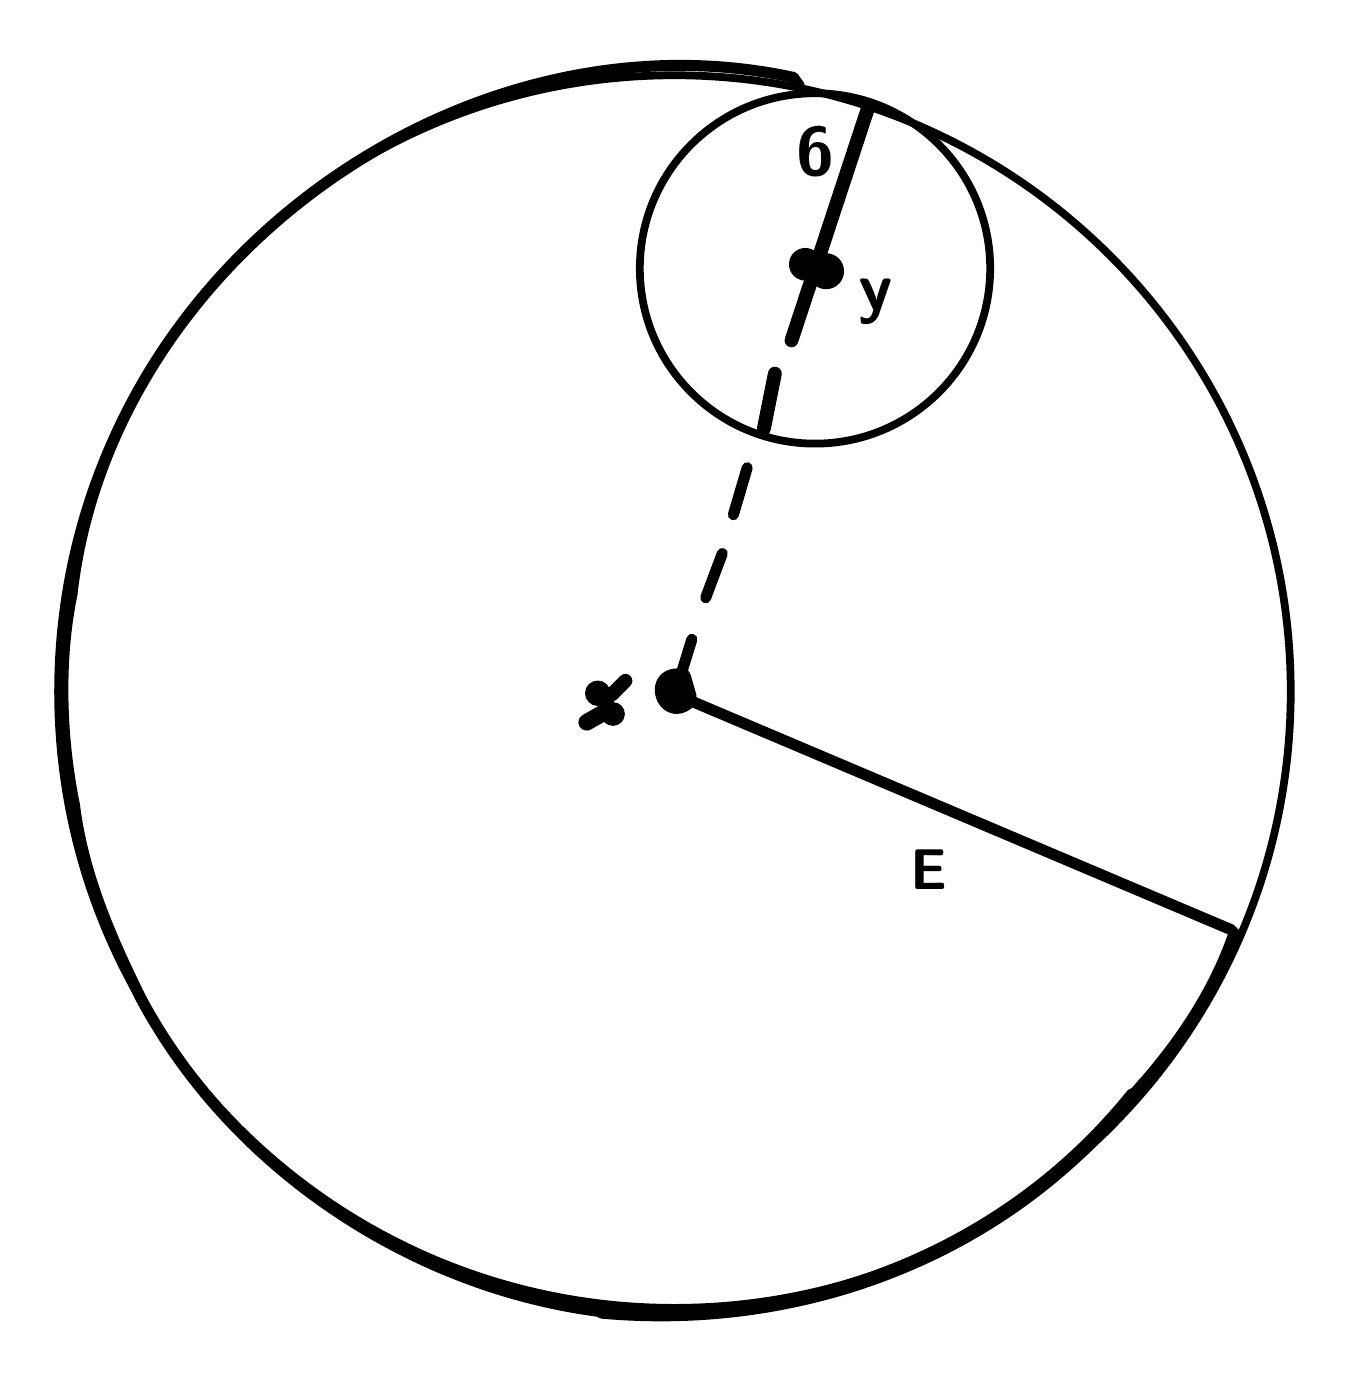
\begin{tikzpicture}[x=1pt, y=-1pt, line width=2.8pt, line cap=round, line join=round]

  %% ════ 填充区（prims2 的 fills）════

  %% ════ 直线段（prims2 的 strokes）════
  \draw[line width=4.0pt] (210.0,242.0) -- (210.0,246.0);
  \draw[line width=5.0pt] (276.0,113.0) -- (304.0,28.0);
  \draw[line width=6.0pt] (209.0,247.0) -- (202.0,251.0);
  \draw[line width=4.0pt] (251.0,190.0) -- (245.0,206.0);
  \draw[line width=5.0pt] (211.0,241.0) -- (216.0,236.0);
  \draw[line width=4.0pt] (236.0,234.0) -- (240.0,221.0);
  \draw[line width=4.0pt] (435.0,326.0) -- (239.0,243.0);
  \draw[line width=3.8pt] (276.8,18.0) -- (279.0,21.0);
  \draw[line width=4.0pt] (255.0,176.0) -- (260.0,159.0);
  \draw[line width=5.0pt] (270.0,125.0) -- (266.0,145.0);
  \draw[line width=7.5pt] (236.0,235.0) -- (238.0,242.0);

  %% ════ 曲线（prims2 的 curves —— 三段式，坐标同为 (y,x)）════
  \draw[line width=4.0pt] (436.0,327.0) .. controls (428.6,348.8) and (415.3,368.3) .. (399.2,385.8);
  \draw[line width=5.0pt] (399.2,385.8) .. controls (353.3,442.8) and (280.9,470.6) .. (207.6,464.0);
  \draw[line width=4.0pt] (207.6,464.0) .. controls (139.8,455.6) and (74.3,413.0) .. (41.0,350.9);
  \draw[line width=4.0pt] (41.0,350.9) .. controls (30.0,328.7) and (20.0,305.8) .. (16.9,280.9);
  \draw[line width=4.0pt] (16.9,280.9) .. controls (12.0,257.0) and (11.0,228.9) .. (16.0,204.7);
  \draw[line width=4.0pt] (16.0,204.7) .. controls (29.7,85.0) and (157.4,-7.9) .. (276.8,18.0);
  \draw[line width=7.0pt] (238.0,243.0) .. controls (230.8,249.0) and (226.0,234.9) .. (235.0,235.0);

  %% ════ 圆 / 椭圆（probe 精测）════
  \draw (233.7,239.9) circle (222.7);
  \draw (284.5,87.0) circle (63.3);

  %% ════ 实心点 ════
  \fill (281.0,85.5) circle (5.9);
  \fill (288.5,88.0) circle (6.5);
  \fill (206.0,240.5) circle (4.6);
  \fill (211.5,248.0) circle (4.3);

  %% ════ 标签（probe 直接给的 \node 行）════
  %% ⚠ 全部补了 fill=white：文字在最上层，否则与曲线交叉干扰
     \node[anchor=center,inner sep=0pt,fill=white,font=\fontsize{31.3}{39.2}\selectfont] at (284.8,44.8) {\textsf{\textbf{6}}};   % box(277,32,14,24)
     \node[anchor=center,inner sep=0pt,fill=white,font=\fontsize{30.5}{38.1}\selectfont] at (306.8,98.8) {\textsf{\textbf{\textit{y}}}};   % box(298,85,17,24)
     \node[anchor=center,inner sep=0pt,fill=white,font=\fontsize{20.7}{25.8}\selectfont] at (325.8,304.2) {\textsf{\textbf{\textit{E}}}};   % box(320,295,12,17)

  % 钉死画布：否则超出的图元/控制点会把页面撑大，1:1 回比就失准
  \pgfresetboundingbox
  \path[use as bounding box] (0,0) rectangle (466,477);
\end{tikzpicture}
\end{document}

% ⚠ 待核清单（probe 拿不准，人眼过一遍）：
%   · 未识别/跳过：⑤ 跳过/未识别的字形
